\documentclass{beamer}
\usepackage{listings}
\lstset{
%language=C,
frame=single, 
breaklines=true,
columns=fullflexible
}
\usepackage{subcaption}
\usepackage{url}
\usepackage{hyperref}
\usepackage{tikz}
\usepackage{graphicx}
\usepackage{ragged2e}
\usepackage{wrapfig}
\usepackage{caption}
\usepackage{subcaption}
\usepackage{tkz-euclide} % loads  TikZ and tkz-base
%\usetkzobj{all}
\usetikzlibrary{calc,math}
\usepackage{float}
\newcommand\norm[1]{\left\lVert#1\right\rVert}
\renewcommand{\vec}[1]{\mathbf{#1}}
\newcommand{\R}{\mathbb{R}}
\newcommand{\C}{\mathbb{C}}
\providecommand{\brak}[1]{\ensuremath{\left(#1\right)}}
\providecommand{\abs}[1]{\vert#1\vert}
\providecommand{\fourier}{\overset{\mathcal{F}}{ \rightleftharpoons}}
\providecommand{\pr}[1]{\ensuremath{\Pr\left(#1\right)}}
\providecommand{\sbrak}[1]{\ensuremath{{}\left[#1\right]}}
\usepackage[export]{adjustbox}
\usepackage[utf8]{inputenc}
\usepackage{amsmath}
\usetheme{Madrid}
\usecolortheme{seahorse}
\settowidth{\leftmargini}{\usebeamertemplate{itemize item}}
\addtolength{\leftmargini}{\labelsep}
\title{Research Paper Presentation}
\author{Taha Adeel Mohammed - CS20BTECH11052}
\institute{IITH(CSE)}
\date{\today}
\begin{document}

\section{Title}
\begin{frame}
\titlepage
\end{frame}

\begin{frame}%{Application of Machine Learning to Lightning Strike Probability Estimation.}
    \begin{block}{Title}
    Application of Machine Learning to Lightning Strike Probability Estimation.
    \end{block}
    \begin{block}{Authors}
    \begin{itemize}
        \item Aderibigbe Adetkitan, Group for Lightning and Overvoltage Protection, Technische Universitaet Ilmenau, Ilmenau, Germany
        \item Michael Rock, Group for Lightning and Overvoltage Protection, Technische Universitaet Ilmenau, Ilmenau, Germany
    \end{itemize}
    \end{block}
    \begin{block}{Year of Publication}
        2020
    \end{block}
\end{frame}

\section{Abstract}
\begin{frame}{Abstract}
    \begin{itemize}
        \justifying
        \item The risk of a lightning strike to a structure is influenced by geometry, the type of material of the structure, and proximity to other structures.
        \item The probability of lightning strike to different points on an object can be determined by applying the concept of probability modulated collection volume using the dynamic electro-geometrical model (DEGM).
        \item The numerical computation of the DEGM is computer resource-intensive and requires extensive programming and analysis to implement, which may be difficult to apply by engineers in the field.
        \item This study explores the feasibility of applying artificial neural network (ANN) and predictive equation-based models developed using data pattern recognition and curve fitting techniques as easy to use alternatives to the numerical DEGM simulations.
    \end{itemize}
\end{frame}

\section{Introduction}
\subsection{Lightning}
\begin{frame}{Introduction}
% \begin{block}{Lightning}
    \begin{itemize}
        \justifying
        \item Lightning is the discharge of transient, high energy current in the atmosphere. The lightning discharge process involves the downward movement of charges referred to as a \textbf{downward leader} via random conducting paths, from the cloud charge centres towards the ground, followed by an upward leader and then an upward return stroke, from the ground towards the cloud.
        \item The risk of a lightning strike to a structure is influenced by geometry, the type of material of the structure, and how it is exposed to lightning strikes relative to other nearby structures.
        \item \textbf{Striking distance} is a term that reflects the extent in terms of geometric distance, from which a point on a structure is exposed to downward leaders and may be struck by lightning. This has been used over time to estimate the protection zone of a lightning rod.
        \item \textbf{Lightning collection volume} is simply the region(volume) above the structure from where downward leaders can strike the structure.
    \end{itemize}
% \end{block}
\end{frame}

\subsection{DEGM and its prerequisites}
\subsubsection{Rolling Sphere lightning protection concept}
\begin{frame}{Introduction}\vspace{-2mm}
\begin{block}{Rolling Sphere lightning protection concept}
    \par \centering \href{run:sls-rolling-sphere-animation.mp4}{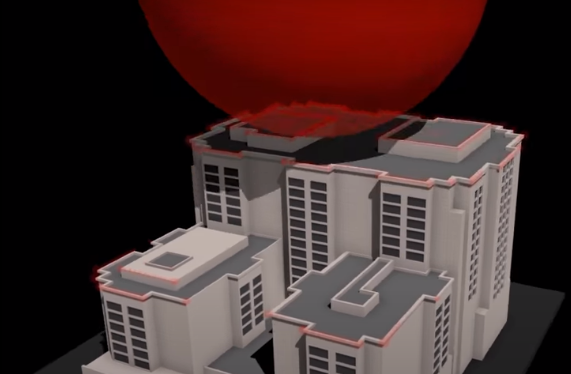
\includegraphics[width=0.4\columnwidth]{Figures/Rolling_sphere.png}}
    \vspace{-2mm}
    \begin{itemize}\justifying
        \item A structure is deemed protected from lightning strikes using the rolling sphere concept if no point on the structure(except lightning rods and the ground) is touched by a sphere of a fixed radius corresponding to a specific protection level.\vspace{-1mm}
        \item However this analysis does not help in identifying high-risk points on the structure as it assumes that the probability of a strike to all points on a structure is the same, and it does not differentiate between strikes to ground, rods and transmission lines as validated by experimental analysis.
    \end{itemize}
\end{block}
\end{frame}

\subsubsection{DEGM}
\begin{frame}{Introduction}
    \begin{block}{DEGM}
    \begin{itemize}
        \justifying
        \item The Dynamic Electro-Geometrical Model(DEGM) is a concept for evaluating the probability of lightning striking a structure, on a point-by-point basis.
        \item By creating meshes on the structure, the probability of strike to diff. points on the meshed structure can be determined using several rolling sphere radii, unlike the rolling sphere concept that uses a fixed radius.
        \item Although the DEGM provides more information for a better design of lightning protection systems for a structure, performing the DEGM analysis may be a major challenge due to the intricate level of programming, and computer resources required as several iterations are performed, which can take a few hours to compute even on advanced simulation computers.
    \end{itemize}
    \end{block}
\end{frame}

\subsubsection{Concept of the DEGM}
\begin{frame}{Introduction}
    \begin{block}{Concept of the DEGM}
    \begin{itemize}
        \justifying
        \item The surface of the structure is meshed into several points to which a downward leader may attach. Also, since downward leaders descend towards the structure from above, spaces above the cuboid within the lightning collection volume of the structure are also meshed into multiple space points, as shown in figure \ref{DEGM_concept}.
        \item For each space point, the nearest surface point(s) on the structure or ground is determined as the likely strike point for any downward leader orientating from that specific point in space.
        \item The effective striking distance for each struck surface point is converted to a probability value by using an appropriate function. The cumulative probability of a lightning strike for each surface point is finally converted to a percentage of the total for the structure.
    \end{itemize}
    \end{block}
\end{frame}

\begin{frame}{Introduction}
    \begin{figure}
        \centering
        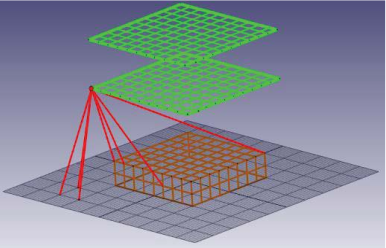
\includegraphics[width=0.7\columnwidth]{Figures/DEGM_concept.png}
        \caption{\centering Illustration of meshed space points above, and surface points on the cuboid structure}
        \label{DEGM_concept}
    \end{figure}
\end{frame}

\subsection{ANN}
\begin{frame}{Introduction}
    \vspace{-2mm}
    \begin{block}{Artificial Neural Network}
    \begin{itemize}
    \justifying
        \item The Artificial Neural Network (ANN) is a computational learning model that mimics the functioning of the neurons of the central nervous system.
        \item The ANN has artificial neurons called nodes, which can be used for evaluating a function based on given inputs, in order to produce a corresponding output.
        \item The nodes are usually interconnected and structured in layers referred to as hidden layers. From the input layer, the output of one neuron will become the input of the next neuron until the final output stage.
    \end{itemize}\vspace{-3mm}
    \begin{figure}
        \centering
        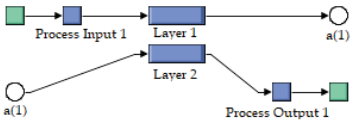
\includegraphics[width=0.5\columnwidth]{Figures/ANN-layers.png}
        \caption{Two layer feed-forward ANN model}
        \label{ANN-layers}
    \end{figure}\vspace{-6mm}
    \end{block}
\end{frame}

\begin{frame}{Introduction}
    \vspace{-1mm}
    \begin{block}{Artificial Neural Network (contd.)}
    \begin{itemize}
    \justifying
        \item The neurons are interconnected by paths with a given weight value (w), which can be adjusted by a learning algorithm that tries to find the best weight value for each path in the model in order to accurately define the output values based on the set of inputs.\vspace{-1mm}
        \item The output of each node is triggered when the weighted input sum is processed by a preset activation function. This gives an output which is equivalent to an electrical potential in biological systems.\vspace{-1mm}
        \item The ANN learning process can be supervised, unsupervised or the hybrid mode, and it is very efficient for modelling non-linear systems.
    \end{itemize}\vspace{-3mm}
    \begin{figure}
        \centering
        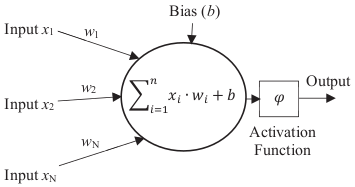
\includegraphics[width=0.35\columnwidth]{Figures/ANN-node.png}\vspace{-1mm}
        \caption{A model of an artificial neuron}
        \label{ANN-node}
    \end{figure}\vspace{-6mm}
    \end{block}
\end{frame}

\section{The Methodology}
\begin{frame}{The Methodology}\vspace{-1mm}
    \begin{itemize}
        \justifying
        \item Two cuboids, Cuboid A and Cuboid B, with different roof surface areas (40m x 40m and 50m x 20m respectively) were considered and analyzed in this study. 
        \item Numerical computations of the DEGM to the two cuboids as a case study was performed using the following heights, 10m, 20m, 30m, 40m and 50m, and the dataset (probability of a strike in percentage for each meshed point on the cuboid) is accumulated from these simulations.
        \item The dataset acquired using heights 10m, 30m, and 50m were used for training and validating the ANN model and equation-based models, and the data-set acquired using heights 20m and 40m were used to further test the extent to which their predictions can be generalized.
    \end{itemize}
    \vspace{-2mm}
    \begin{figure}
        \centering
        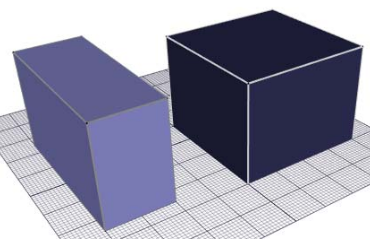
\includegraphics[width=0.28\columnwidth]{Figures/Cuboid_A_B.png}
        \caption{Cuboid A and Cuboid B}
        \label{Cuboid_A_B}
    \end{figure}
\end{frame}

\begin{frame}{The Methodology}
    \begin{itemize}
        \justifying
        \item To apply machine-learning techniques to a dataset, the inputs and outputs of the model must be well defined.
        \item In this case, the desired \textbf{output} is the \textbf{percentage probability of a strike to each point}(hereby referred to as target), which has been determined by DEGM analysis.
        \item There is a need to define the input features as independent variables that will define the desired output. To do this, attributes of the cuboid and the DEGM as a concept were considered to generate seven input features, as defined in the following section.
    \end{itemize}
\end{frame}

\begin{frame}{}
    \begin{block}
    \justifying
        \;\;\;\;\;\;\; Firstly, the surface points on the cuboid structure were classified into five different types: sidewall (SW), corner (C), wall edge (WE), inner roof (IR), and roof edge (RE).
        \begin{figure}
            \centering
            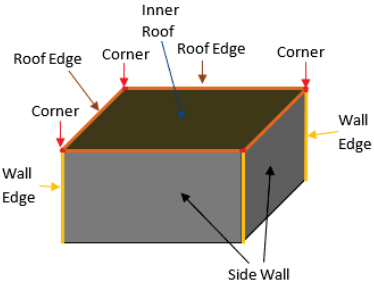
\includegraphics[width=0.5\columnwidth]{Figures/Surface_pts.png}
            \caption{Types of surface points}
            \label{Surface_pts}
        \end{figure}
    \end{block}
\end{frame}

\section{Input Features}
\begin{frame}{Input Features}
    \begin{block}{Feature A}
    \justifying
        \begin{wrapfigure}{r}{0.3\columnwidth}
            \centering\vspace{-5mm}
            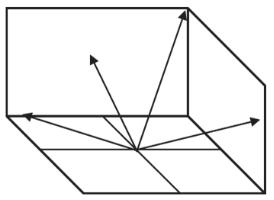
\includegraphics[width=0.26\columnwidth]{Figures/Feature_A.png}
            \label{Feature_A}
        \end{wrapfigure}
        \vspace{1mm}This is the distance between each surface point and a reference point at the centre of the cuboid on the ground level. This parameter measures the relative displacement of each surface point from the datum point.
    \end{block}
    \begin{block}{Feature B}
    \justifying
        \begin{wrapfigure}{r}{0.3\columnwidth}
            \centering\vspace{-6mm}
            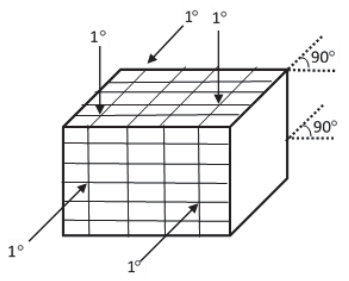
\includegraphics[width=0.28\columnwidth]{Figures/Feature_B.png}
            \label{Feature_B}
        \end{wrapfigure}
         \vspace{2mm}This reflects the exposure of each type of surface points in angular terms using a single horizontal surface as a reference plane at each object height. For corners and wall edges, the exposure angle is 90°, while it is 1° for all other points.\vspace{3mm}
    \end{block}
\end{frame}

\begin{frame}{Input Features}
    \begin{block}{Feature C}
    \justifying
        Height of each discretized surface point above the ground.
    \end{block}
    \begin{block}{Feature D}
    \justifying
        The type of surface point coded as follows: 1 for the SW, 2 for the WE, 3 for the C, 4 for the RE, and 5 for the IR.
    \end{block}
    \begin{block}{Feature E}
    \justifying
        The surface area of the cuboid's roof(exposed top) in m$^2$
    \end{block}
    \begin{block}{Feature F}
    \justifying
        The height of the cuboid.
    \end{block}
    \begin{block}{Feature G}
    \justifying
        The total surface area of the four cuboid sides in m$^2$
    \end{block}
\end{frame}

\section{The ANN Model}
\subsection{The Model}
\begin{frame}{The ANN Model}
    \begin{itemize}
        \justifying
        \item To achieve an ANN-based DEGM, a \textbf{seven input} neural network model was developed using a \textbf{two-layer} feed-forward network comprising of \textbf{18 neurons}.
        \item The dataset containing \textbf{36900 samples} (e.g. $A = 29.4618,\, B=1,\, C= 12,\, D=SW,\, E = 1600,\, F = 30, \text{ and } G = 4800$) was randomly divided into three in the ratio, $70\%$ for training, $15\%$ for performance evaluation, and the remaining $15\%$ for testing.
        \item The model was trained using the \textbf{Levenberg-Marquardt optimization algorithm} for \textbf{supervised learning} using the backpropagation rule.
        \item The analysis was carried out using the neural fitting tool on \textbf{MATLAB}.
        \item The training process is performed iteratively by feeding the inputs, updating the neural weights, and getting an output repeatedly until a preset limit is attained. Each of this iteration is referred to as an epoch, and in this study, the iteration was terminated after \textbf{1000 epochs}.
    \end{itemize}
\end{frame}

\subsection{Results}
\subsubsection{Training progress report}
\begin{frame}{The ANN Model - Results}
    The simulation (training, validation, and testing) was completed in 2 minutes. The training status of the ANN model after completion is shown below
    \begin{figure}
        \centering
        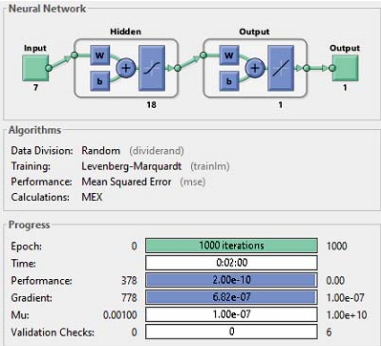
\includegraphics[width=0.5\columnwidth]{Figures/ANN-report.png}
        \caption{The Artificial Neural Network and training progress report}
        \label{ANN-report}
    \end{figure}
\end{frame}

\subsubsection{Error Histogram}
\begin{frame}{The ANN Model - Results}
    \vspace{-2mm}
    \begin{block}{Error Histogram}
    \begin{itemize}
    \justifying
        \item The error histogram is a plot of the error distribution, and it shows that highest error is around the central value of $5.09 \times 10^{-6}$, and the error decreases on both sides of the maximum error point, and this is a good indication of minimal predictive error.\vspace{-1mm}
        \item The performance of the model was evaluated using the \textbf{mean square error}(MSE) and \textbf{regression R$^2$ value}.
    \end{itemize}\vspace{-3mm}
    \begin{figure}
        \centering
        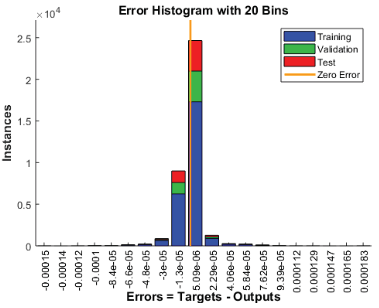
\includegraphics[width=0.38\columnwidth]{Figures/Error-histogram.png}\vspace{-2mm}
        \caption{Error histogram}
        \label{Error-histogram}
    \end{figure}\vspace{-6mm}
    \end{block}
\end{frame}

\subsubsection{Mean Square Error}
\begin{frame}{The ANN Model - Results}
\vspace{-1.5mm}
\begin{block}{Mean Square Error(MSE)}
    \begin{itemize}
        \justifying
        \item \;
        % If $n$ is sample size, $Y_i$ is observed value, and $\hat{Y_i}$ is predicted value, then\vspace{-3.5mm}
        \vspace{-6mm}\begin{align*}
            \text{MSE}=\dfrac{1}{\text{Sample Size(n)}}\times \sum_{i=1}^n(\text{Observed value}_i-\text{Predicted value}_i)^2
        \end{align*}\vspace{-6.5mm}
        \item The lower the MSE, the better the result. For the training process, the MSE observed is $2.000 \times 10^{-10}$, $2.103 \times 10^{-10}$ for validation, and $2.138 \times 10^{-10}$ for the testing.\vspace{-1mm}
        \item The performance validation in terms of the reduction of the MSE with successive iterations is shown below.
    \end{itemize}\vspace{-3mm}
    \begin{figure}
        \centering
        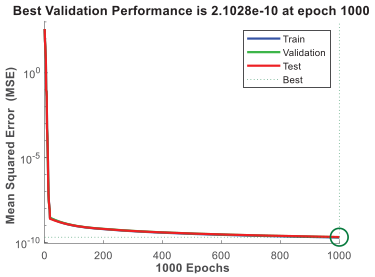
\includegraphics[width=0.35\columnwidth]{Figures/MSE-trend.png}\vspace{-2mm}
        \caption{MSE trend}
        \label{MSE-trend}
    \end{figure}\vspace{-6mm}
    \end{block}
\end{frame}

\subsubsection{Regression values}
\begin{frame}{The ANN Model - Results}
    \begin{block}{Regression $R^2$ value}
        \begin{itemize}
            \justifying
            \item $R^2$ is a statistical measure of fit that indicates how much variation of a dependent variable is explained by the independent variable(s) in a regression model.
            \item \; \vspace{-6mm} \begin{align*}
                R^2 = 1 - \dfrac{\text{Unexplained Variation}}{\text{Total Variation}}\vspace{-4mm}
            \end{align*}
            \item $R^2$ values are in the range from $0$ to $1$. Higher the $R^2$ value,the better the model results.
            \item The graphs on the next slide show the regression plots for training, validation, testing and the overall model performance.
            \item  An \textbf{overall R$^{\textbf{2}}$ value of 1 was achieved}, which indicates a good model fit.
        \end{itemize}
    \end{block}
\end{frame}

\begin{frame}{The ANN Model - Results}
    \begin{block}{Regression Plots}
    \begin{figure}
         \centering
         \begin{subfigure}[b]{0.23\textwidth}
             \centering
             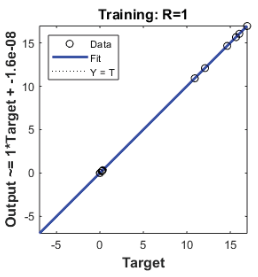
\includegraphics[width=\textwidth]{Figures/Regression-training.png}
             \caption{\centering Regression plot for the training data}
         \end{subfigure}
         \hfill
         \begin{subfigure}[b]{0.23\textwidth}
             \centering
             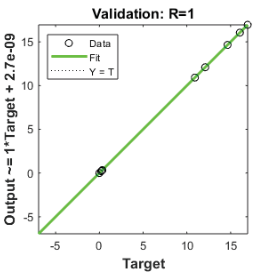
\includegraphics[width=\textwidth]{Figures/Regression-validation.png}
             \caption{\centering Regression plot for the validation data}
         \end{subfigure}
         \hfill
         \begin{subfigure}[b]{0.23\textwidth}
             \centering
             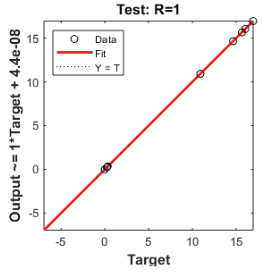
\includegraphics[width=\textwidth]{Figures/Regression-test.png}
             \caption{\centering Regression plot for the test data}
         \end{subfigure}
         \hfill
         \begin{subfigure}[b]{0.23\textwidth}
             \centering
             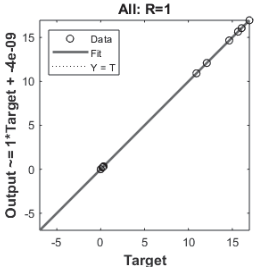
\includegraphics[width=\textwidth]{Figures/Regression-all.png}
             \caption{\centering Regression plot for the overall model}
         \end{subfigure}
    \end{figure}
    \end{block}
\end{frame}

\subsubsection{Overview}
\begin{frame}{The ANN Model - Results}
    \begin{block}{Overview}
    \justifying
        For an overview of the predictive ability of the ANN model, some samples of the predictions for Cuboid A, and Cuboid B from the five cuboid heights, i.e. 10 m, 20 m, 30 m, 40 m, 50 m are presented below
        \begin{figure}
         \centering
         \begin{subfigure}[b]{0.32\textwidth}
             \centering
             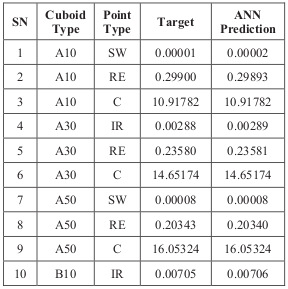
\includegraphics[width=\textwidth]{Figures/ANN-overview1.png}
         \end{subfigure}
         \hfill
         \begin{subfigure}[b]{0.32\textwidth}
             \centering
             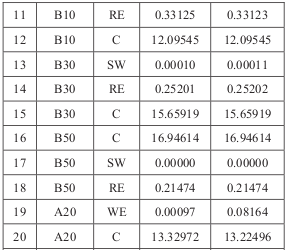
\includegraphics[width=\textwidth]{Figures/ANN-overview2.png}
         \end{subfigure}
         \hfill
         \begin{subfigure}[b]{0.32\textwidth}
             \centering
             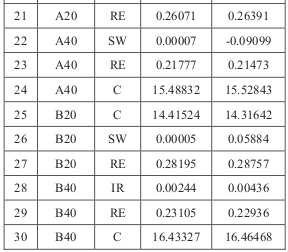
\includegraphics[width=\textwidth]{Figures/ANN-overview3.png}
         \end{subfigure}
         \caption{Comparison of the predicted results with the target value}
    \end{figure}
    \end{block}
\end{frame}

\begin{frame}{The ANN Model - Results}
    \begin{block}{Overview(contd.)}
    \begin{itemize}\justifying
        \item The results from serial number 1 to 18 are from samples used in the ANN model development, i.e. 10 m, 30 m, and 50 m.
        \item In order to evaluate the ability of the model to predict for new data, data samples from 20 m, and 40 m, both for Cuboid A and Cuboid B which were not part of the ANN model development process were analyzed, and the results for few samples are shown comparatively from serial number 19 to 30.
        \item Although the predictions are not perfect, the result shows a close approximation to the target, especially for the roof edge (RE), the internal roof (IR), and the corner (C) points.
    \end{itemize}
    \end{block}
\end{frame}

\section{The Equation-based Models}
\subsection{The Model}
\begin{frame}{Equation-based Model}
    \begin{itemize}\justifying
        \item As an alternative to the ANN approach, the possibility of deploying equations that reasonably model the attributes of the dataset for predictive analysis was explored.
        \item Only three key features were considered in the model, and these are feature A, feature C, and feature F. The addition of more features, only made the equations more complex without significant improvement in accuracy.
        \item Separate equations and analysis were developed for each type of surface point, i.e. WE, SW, RE, IR, and C, by exploring data fitting techniques using \textbf{ndCurveMaster}.
        \item Unlike the analysis for ANN, where the percentage of the probability of lightning strike was directly predicted, for the first equation-based model, the probability modulated collection volume(PMCV) (collection volume(which is infinite) is modulated to be 1 for roof surface points, and relative to that for other surface points.) will be predicted, and this will be converted to a percentage at the end of the analysis.
    \end{itemize}
\end{frame}

\subsection{Results}
\subsubsection{The equations for diff surface points}
\begin{frame}{Equation-based Model - Results}\vspace{-1mm}
    \justifying
    For each of our different surface point types, we have an equation describing the predictive model for computing the PMVC for a surface point of that type, using variables A, C and F as inputs, and a figure presenting a visual view of the extent to which the predicted values are well fitted to the actual PMCV values.
    
    \begin{block}{Corner surface points}
        \;\vspace{-5mm}\begin{align}
            CornerP = k_0 + k_1 \times C^11 + k_2 \times F^0.85,
        \end{align}\\\vspace{-3mm}\justifying
        where $k_0 = -461.24$, $k_1 = 5.6101 x 10^{-17}$, $k_2 = 305.341$, and CornerP is the PMCV of one corner surface point.\vspace{-2mm}
        \begin{figure}
            \centering
            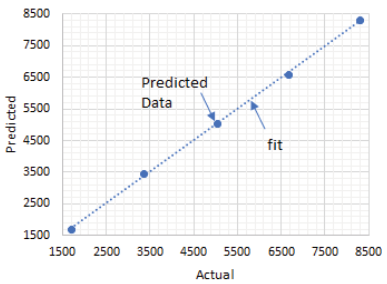
\includegraphics[width=0.3\columnwidth]{Figures/Eq-Corner.png}\vspace{-1mm}
            \caption{A fit of the predicted vs actual PMCV for corner points}
        \end{figure}\vspace{-6.5mm}
    \end{block}
\end{frame}

\begin{frame}{Equation-based Model - Results}
    \begin{block}{Roof edge surface points}
        \;\vspace{-5mm}\begin{multline}
            RoofEdgeP = j_0 + j_1 \times C^4 + j_2 \times F^{2.4} + j_3 \times A^{0.93} \times C^{0.82}\\ + j_4 \times A^{0.27} \times C^{1.2} \times F^{0.4},
        \end{multline}\\\vspace{-3mm}\justifying
        where $j_0 = 42.899$, $j_1=-1.9446 \times 10^{-5}$, $j_2 = 0.01538$, $j_3 = -2.176 \times 10^{-14}$, $j_4 = 5.862 \times 10^{-14}$, and RoofEdgeP is the PMCV of one roof edge surface point.\vspace{-2mm}
        \begin{figure}
            \centering
            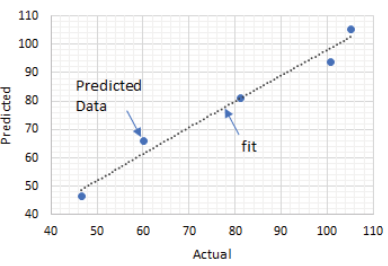
\includegraphics[width=0.3\columnwidth]{Figures/Eq-RE.png}\vspace{-1mm}
            \caption{A fit of the predicted vs actual PMCV for roof edge points}
        \end{figure}\vspace{-6.5mm}
    \end{block}
\end{frame}

\begin{frame}{Equation-based Model - Results}
    \begin{block}{Wall edge surface points}
        \;\vspace{-5mm}\begin{multline}
            WallEdgeP = m_0 + m_1 \times e^{2A} + m_2 \times C^{3.75} + m_3 \times e^{5F}\\ + m_4 \times A^{-0.083} \times C^{4.8} + m_5 \times 2^{A} \times F^{-5.25}\\ + m_6 \times C^{2.75} \times F^{0.01} + m_7 \times A^{-1.6} \times C^{10} \times F^{0.66},
        \end{multline}\\\vspace{-3mm}\justifying
        where $m_0 = 0.001029$, $m_1 = 2.7843 \times 10^{-51}$, $m_2 = 9.03 \times 10^{-6}$, $m_3 = 1.367 \times 10^{-112}$, $m_4 = -1.251 \times 10^{-7}$, $m_5 = -5.009 \times 10^{-10}$, $m_6 = -5.57 \times 10^{-5}$, $m_7 = 4.199 \times 10^{-16}$, and WallEdgeP is the PMCV of one wall edge surface point.\vspace{-2mm}
        \begin{figure}
            \centering
            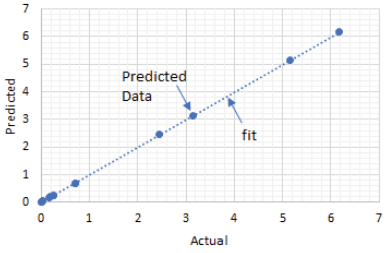
\includegraphics[width=0.3\columnwidth]{Figures/Eq-WE.png}\vspace{-1mm}
            \caption{A fit of the predicted vs actual PMCV for wall edge points}
        \end{figure}\vspace{-6.5mm}
    \end{block}
\end{frame}

\begin{frame}{Equation-based Model - Results}\vspace{-1mm}
    \begin{block}{Sidewall surface points}
        \;\vspace{-5mm}\begin{multline}
            SideWallP = n_0 + n_1 \times A^{14} + n_2 \times C^{4.25} + n_3 \times F^{1.8}\\ + n_4 \times A^{0.083} \times C^{0.69} + n_5 \times A^{15} \times F^{-3.3}\\ + n_6 \times C^{2.05} \times F^{0.067} + n_7 \times A^{0.01} \times C^{1.6} \times F^{0.1},
        \end{multline}\\\vspace{-3mm}\justifying
        where $n_0 = -2.9218 \times 10^{-4}$, $n_1 = -4.0327 \times 10^{-27}$, $n_2 = -2.6635 \times 10^{-9}$, $n_3 = 3.5299 \times 10^{-7}$, $n_4 = 0.00036794$, $n_5 = 3.0598 \times 10^{-23}$, $n_6 = 0.00008559$, $n_7 = -2.2560 \times 10^{-4}$, and SideWallP is the PMCV of one roof edge surface point.\vspace{-2.7mm}
        \begin{figure}
            \centering
            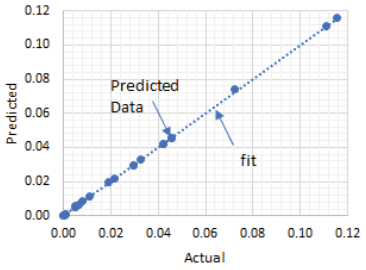
\includegraphics[width=0.3\columnwidth]{Figures/Eq-SW.png}\vspace{-1mm}
            \caption{A fit of the predicted vs actual PMCV for sidewall points}
        \end{figure}\vspace{-6.5mm}
    \end{block}
\end{frame}

\begin{frame}{Equation-based Model - Results}
    \begin{block}{Inner roof surface points}
    \begin{itemize}\justifying
        \item This is the inner part of the roof which are exposed to vertical lightning strikes from space points directly above this region.
        \item The PMCV of each inner roof surface point should be 1.0, but in the computation of the DEGM, the analysis was performed up to $300$ m (not $\infty$) above the roof, and the resulting PMCV is \textbf{0.991}. The value is constant for all inner roof surface points
    \end{itemize}
    \end{block}
\end{frame}

\begin{frame}{Equation-based Model - Results}
    \begin{block}{CubeSideP}
    \begin{itemize}\justifying
        \item The value of the PMCV for each of the sidewalls and wall edge surface points are quite small in value, with some values in the order of $10^{-8}$, and these small values were difficult to accurately predict by the model.
        \item A relationship between the PMCV of a corner point which was predicted accurately and the total PMCV of all surface points on the four side faces of the cuboid structure (i.e. CubeSideP) was developed as shown in (5).
        \vspace{-7.5mm}\begin{multline}
            CubeSideP = z_0\! +\! z_1\! \times\! CornerP^{3.8}\! +\! z_2 \!\times\! E^{4}\! +\! z_3\! \times\! G^{3.45}\! +\! z_4\! \times\! \ln^4 F,
        \end{multline}\\\vspace{-1.5mm}
        where $z_0 = 3.4407$, $z_1 = 6.681 \times 10^{-13}$, $z_2= -4.4417 \times 10^{-14}$, $z_3 = 3.3648 \times 10^{-2}$, and $z_4= -0.15141$.
        \item The total probability of a strike to the four sides of the cuboid structures, is typically less than $1.3\%$ of the total probability, while surface points on the roof and corners account for the rest.
    \end{itemize}
    \end{block}
\end{frame}

\subsubsection{Total PMVC}
\begin{frame}{Equation-based Model - Results}
    \begin{block}{Total PMCV}
    \begin{itemize}\justifying
        \item The total PMCV for the whole structure is required to convert the results obtained using (1) to (4) to percentage probability values.
        \item The total PMCV is simply the summation of the PMCVs for all the corner points, the wall edge points, roof edge points, the four sidewall points (i.e. CubeSideP), and the inner roof. This can be computed using (6), where L is the length and B is the breadth of the cuboid.
        \vspace{-4mm}\begin{multline}
            Total\ PMCV =  4 \times CornerP+(2L + 2B-4) \times RoofEdgeP\\+ (L-1)\times(B-1)\times 0.991 + CubeSideP
        \end{multline}\\\vspace{-3mm}
    \end{itemize}
    \end{block}
\end{frame}

\subsubsection{Percentage Probability}
\begin{frame}{Equation-based Model - Results}
    \begin{block}{Percentage Probability}
        Our desired output (percentage probability of a strike to each point) can now be computed from the below formulae.
        \setlength{\jot}{9pt}
        \begin{align}
            \text{Corner Probability(\%)} &= \dfrac{CornerP\times100}{Total\ PMCV}\\
            \text{Roof Edge Probability(\%)} &= \dfrac{RoofEdgeP\times100}{Total\ PMCV}\\
            \text{Inner Roof Probability(\%)} &= \dfrac{0.991\times100}{Total\ PMCV}\\
            \text{Side Wall Probability(\%)} &= \dfrac{SideWallP\times100}{Total\ PMCV}
        \end{align}
    \end{block}
\end{frame}

\subsubsection{Direct Equation}
\begin{frame}{Equation-based Model - Results}
    \begin{block}{Direct Equation}
    \begin{itemize}\justifying
       \item Further, an equation for directly predicting the percentage probability(target) of a lightning strike to the roof edge, corner, and inner roof area was developed. 
       \item The sidewall and the wall edges were excluded from the analysis because of their small strike probability which reduces the accuracy of a general equation for all the five types of points.
       \item The result is directly in percentage using (11), and this is an alternative to the indirect analysis by calculating PMCV, and it applies A, B, C, D, and E as input variables.\vspace{-2mm}
       \begin{align}
           \text{Target (\%)} = Q_1+Q_2+Q_3+Q_4,
       \end{align}\\\vspace{-3mm}
       where $Q_1$, $Q_2$, $Q_3$, and $Q_4$ are defined on the next slide.
 \end{itemize}
    \end{block}
\end{frame}

\begin{frame}{Equation-based Model - Results}\vspace{-2mm}
    \begin{block}{Direct Equation(contd.)}\vspace{-6.2mm}
        \begin{multline*}
            Q_{1}=t_{0}+t_{1} \cdot B^{0.24}+t_{2} \times C^{-2}+t 3 \times D^{5.9}+t_{4} \times E^{0.96}\\+t_{5} \times A^{2.95} \times B^{3.25}+t_{6} \times A^{3.35} \times 6^{-C}+t_{7} \times A^{5} \times D^{4}
        \end{multline*}\vspace{-12mm}
        \begin{multline*}
            Q_{2}=t_{8} \times A^{1.55} \times E^{0.22}+t_{9} \times B^{0.32} \times C^{-3.2}+t_{10} \times B^{0.77} \times E^{0.18} +t_{11}\\ \times C^{-5.25} \times D^{16}+t_{12} \times C^{3.55} \times E^{0.44}+t_{13} \times \ln ^{3} D \times E^{0.167}
        \end{multline*}\vspace{-12mm}
        \begin{multline*}
            Q_{3}=t_{14} \times A^{1.1} \times B^{4.8} \times C^{-2.75}+t_{15} \times B^{0.97} \times C^{3.4} \times D^{-4.9}+t_{16} \times C^{-0.125}\\ \times D^{-5.55} \times E^{-0.65}+t_{17} \times A^{0.09} \times B^{-4.9} \times C^{2.75} \times 7^{-D}
        \end{multline*}\vspace{-12mm}
        \begin{multline*}
            Q_{4}=t_{18} \cdot B^{-2.8} \cdot C^{0.07} \cdot D^{-1.45} \cdot E^{6} + t_{19} \cdot A^{0.27} \cdot B^{2.75} \cdot C^{-2.5} \cdot D^{0.8} \cdot E ^ {3.25}
        \end{multline*}\;\\\vspace{-7.5mm}\justifying
        Where $\mathrm{t}_{0}=-8.6018$, $\mathrm{t}_{1}=9.838205$, $\mathrm{t}_{2}=-27.930$,  $\mathrm{t}_{3}=0.0001855$, $\mathrm{t}_{4}=0.0012095$,  $\mathrm{t}_{5}=2.1612 \times 10^{-11}$, $ \mathrm{t}_{6}=-0.088903$, $\mathrm{t}_{7}=-4.351 \times 10^{-16}$, $\mathrm{t}_{8}=1.2513 \times 10^{-7}$, $\mathrm{t}_{9}=379.82078$,  $\mathrm{t}_{10}=-0.08143$, $\mathrm{t}_{11}=9.097 \times 10^{-9}$, $\mathrm{t}_{12}=6.811 \times 10^{-12}$, $\mathrm{t}_{13}=-0.34028$, $\mathrm{t}_{14}=-2.398 \times 10^{-8}$, $ \mathrm{t}_{15}=-1.8685 \times 10^{-5}$,  $\mathrm{t}_{16}=185702.9, \mathrm{t}_{17}=-1.466 \times 10^{-4}, \mathrm{t}_{18}=-4.4026 \times 10^{-20}$, and $\mathrm{t}_{19}=2.242 \times 10^{-15} .$
    \end{block}
\end{frame}

\subsubsection{Overview}
\begin{frame}{Equation-based Model - Results}\vspace{-1.5mm}
    \begin{block}{Overview}
    \begin{itemize}\justifying
        \item Results from serial no. 1 to 18 are from samples used in the development of equations(from 10m, 30m, and 50m high cuboids), and results from 19 to 30 are from new surface points(from 20m and 40m high cuboids) to overview the ability of the model to predict for new data points.\vspace{-1mm}
        \item From the results, it is observed that the model was able to predict close results for samples used in developing the models, while for new data samples, there were slight deviations from the expected values.
    \end{itemize}
        \begin{figure}\vspace{-3mm}
         \centering
         \begin{subfigure}[b]{0.325\textwidth}
             \centering
             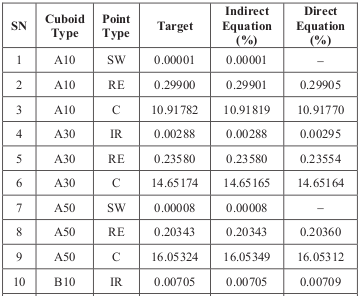
\includegraphics[width=\textwidth]{Figures/Eq-overview1.png}
         \end{subfigure}
         \hfill
         \begin{subfigure}[b]{0.325\textwidth}
             \centering
             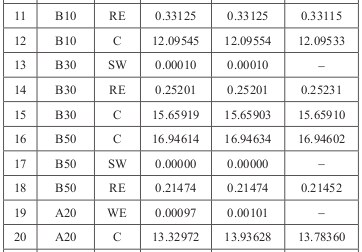
\includegraphics[width=\textwidth]{Figures/Eq-overview2.png}
         \end{subfigure}
         \hfill
         \begin{subfigure}[b]{0.325\textwidth}
             \centering
             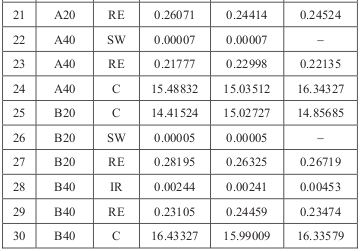
\includegraphics[width=\textwidth]{Figures/Eq-overview3.png}
         \end{subfigure}\vspace{-1mm}
         \caption{Comparison of the predicted results using equations with the target value}
    \end{figure}\;\\\vspace{-28pt}
    \end{block}
\end{frame}

\section{Conclusion}
\begin{frame}{Conclusion}
    \begin{block}{}
        \begin{itemize}\justifying
            \item Accurate design of lightning protection systems  is vital for ensuring the safety of lives and properties. Air-termination networks must be positioned at high-risk points on a structure to ensure optimal lightning interception.
            \item The ANN model developed was able to show close approximations to expected results from DEGM with an overall regression R$^2$ value of 1.
            \item In terms of the ability of the models developed to predict accurate results for unfamiliar data samples, the ANN model performed far better than the equation-based model in predicting results for surface points on new cuboid structures.
        \end{itemize}
    \end{block}
\end{frame}


\end{document}